\documentclass[10pt]{article}
\setlength{\parskip}{0.25\baselineskip}
\usepackage[margin=1in]{geometry} 
\usepackage{amsmath,amsthm,amssymb, graphicx, multicol, array}
\usepackage[font=small,labelfont=bf]{caption}
 
\newenvironment{problem}[2][Problem]{\begin{trivlist}
\item[\hskip \labelsep {\bfseries #1}\hskip \labelsep {\bfseries #2.}]}{\end{trivlist}}

\begin{document}
 
\title{First Assignment}
\author{Eric Tao\\
Math 240: Homework \#2}
\maketitle
 
\begin{problem}{2.1}

Show that the union of the coordinate axes in $\mathbb{A}^3$ is a closed algebraic set, and determine generators for its ideal.

\end{problem}

\begin{proof}[Solution]

Here, we will use $x,y,z$ to denote the coordinates in $\mathbb{A}^3$, and call the union of the coordinate axes $C$. Suppose a point is in the zero set of the polynomials $Z(\{xy,yz,xz\})$. Since $xy = 0$, suppose we are in the case $x = 0$. Then $xz = 0$ automatically, and just need $yz = 0$. Then the cases would be either $x,y = 0$ or $x,z = 0$, which are the $z$-axis and the $y$-axis respectively. Repeating this argument for the other cases, we can also recover the $y$-axis. Then, we have that a point in the zero set has to be on one of the coordinate axes, and $Z(\{xy,yz,xz\}) \subseteq C$.

Now, suppose we have a point on a coordinate axis. Then, at least 2 of the coordinates must be 0. But then, $xy,yz,xz = 0$ and we have that $C \subseteq Z(\{xy,yz,xz\})$ and thus $C = Z(\{xy,yz,xz\})$. Since the union of the coordinate axes is the zero set of a set of polynomials, it must be a closed algebraic set, and we may take the ideal $<xy,yz,xz>$.

\end{proof}

\begin{problem}{2.2}

Consider the curve $C$ in $\mathbb{A}^3$ given in parametric form by $(t,t^2,t^3)$. Show that $C$ is an algebraic set and determine generators for the (radical) ideal of $C$.

\end{problem}

\begin{proof}[Solution]

Consider the zero set of the polynomials $f = y- x^2$ and $g = z - x^3$, $Z(f,g)$. If we have a point on $C$, we can express it as $(t_0, t_0^2, t_0^3)$ for some $t_0 \in k$. Then, we have that $f(t_0,t_0^2,t_0^3) = t_0^2 - (t_0)^2 = 0$ and $g(t_0,t_0^2,t_0^3) = t_0^3- (t_0)^3 = 0$, and thus $C \subseteq Z(f,g)$.

Now, suppose we have a point on $Z(f,g)$. Then, we have that $y - x^2 = 0, z - x^3 = 0 \implies y = x^2, z = x^3$. Fix a point $x_0 \in k$, then we have that the points have form $(x_0,x_0^2,x_0^3)$. But these are exactly the points on $C$. So, $Z(f,g) \subseteq C$, and $C = Z(f,g)$. Since $C$ is the zero set of some polynomials in $k[x,y,z]$, C is an algebraic set, and we can take $<f,g>$ as an ideal of $C$. 

Now, consider the map from $h: k[x,y,z] \to  k[x,z]$ via $y \to x^2$. It is clear that this is surjective, so we need only prove that $\ker(h) = <y-x^2>$. It is clear that $<y - x^2> \subseteq \text{ker}(h)$. Take $j \in \ker(h)$. We may rewrite the polynomial $j(x,y,z) = \Sigma_{k=0}^n j_k(xz) y^n$. If we do a rescaling, as in class, then we can rewrite this polynomial taking $y \to y-x^2 + x^2$, and we find $j(x, y-x^2 + x^2,z) = \Sigma_{k=0}^n j_k(xz) [ (y-x^2) + x^2]^n$. Multiplying out, and regrouping terms, we can group terms as $j = \Sigma_{k=0}^n j'_k(xz) [ (y-x^2)]^n$. In particular, since for each power $n \geq 1$, the term goes to $0$ when $y \to x^2$, it must have constant term $0$. Then, we have that $\ker{h} = <y-x^2>$ as $y - x^2$ divides every term of $j$, and $j$ was a generic polynomial. So, we have that $h$ is an isomorphism.

Without going through every step, we can see that the same argument will work for $m: k[x,z] \to k[x]$ where $z \to x^3$ with $\ker{m} = <z - x^3>$. Then, we notice that the kernel of $m \cdot h$ is just the ideal generated by $<\ker{h},\ker{m}>$, which we can write in terms of our generators, $< z - x^3, y-x^2>$. But, the composition of two isomorphisms is itself an isomorphism, so we have that this ideal is the kernel of a isomorphism to an integral domain, therefore prime, therefore radical.
\end{proof}

\begin{problem}{2.3}

(a) Consider the set of four points in $X = \{(0,0),(0,1),(1,0),(1,1)\} \subseteq \mathbb{A}^2$. Find generators for its ideals.

(b) Do the same for the points $Y = \{(0,0),(0,1),(1,1),(2,2)\}$. What is the difference between the two cases, and why?

\end{problem}

\begin{proof}[Solution]

(a) We notice that we can think of this zero set as the intersection of the zero sets of the lines $x, x-1$ and $y, y-1$. We can also think of, for example, $x, x-1$ as the union of the zero sets of $x$, $x-1$. Then, from proposition 2.1.6 from Osserman, we have:

$$ Z(\{x\}) \cup Z(\{x-1\}) = Z(\{x(x-1)\}) $$

and

$$ Z(\{x(x-1)\}) \cap Z(\{y(y-1)\}) = Z(\{x(x-1),y(y-1)\})$$

Now, we notice that $Z(\{x\}) = \{ (0,y) \}$ and  $Z(\{x-1\}) = \{ (1,y) \}$, so we have that $Z(\{x(x-1)\}) = \{ (x,y) : x = 0,1 \}$ and analogously for $y$.

Then, $Z(\{x(x-1)\}) \cap Z(\{y(y-1)\}) = \{ (x,y) : x = 0,1 \} \cap  \{ (x,y) : y = 0,1 \} = \{ (x,y) : x,y = 0,1 \} = X$. Thus we have that $Z(\{x(x-1),y(y-1)\}) = X$, and thus we can take our ideal as $<x(x-1),y(y-1)> \subseteq k[x,y]$.

(b) Working analgously, we can see that we can take this as the intersection of the union of sets of lines again. In particular, we will take the following zero sets:

$$Z_1 = Z(\{x(y-1)(1/2x + 1)\})$$

and 

$$ Z_2 = Z(\{(y-x)(y-x-1)\})$$

\begin{minipage}{0.30\linewidth}
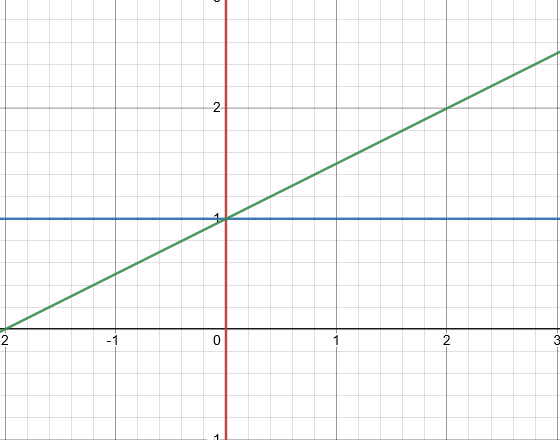
\includegraphics[width=\linewidth]{z_1_lines}
\captionof{figure}{The lines $x = 0$, $y = 1$, and $y = \frac{x}{2} + 1$.}
\end{minipage}
\begin{minipage}{0.30\linewidth}
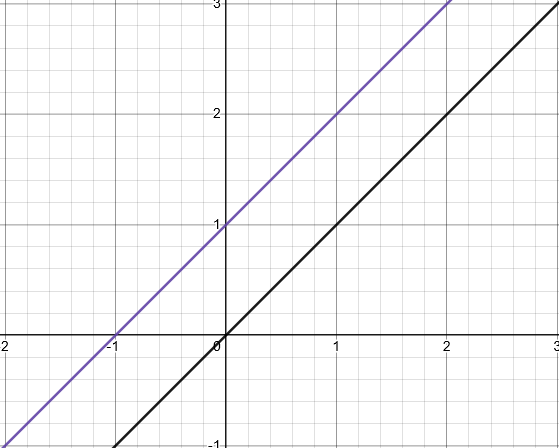
\includegraphics[width=\linewidth]{z_2_lines}
\captionof{figure}{The lines $y = x$ and $y = x+1$.}
\end{minipage}
\begin{minipage}{0.30\linewidth}
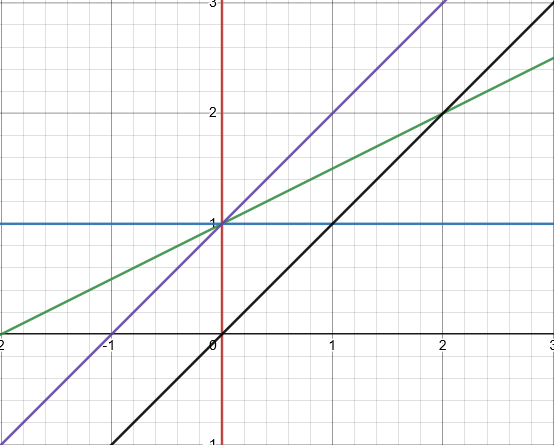
\includegraphics[width=\linewidth]{both_lines}
\captionof{figure}{All lines in the previous 2 figures.}
\end{minipage}

Let's justify this a little bit. We note that because lines can only meet in $0,1$ or infinitely many points, we are guaranteed that these are the only points of intersection for our zero set, and we claim by picture that $ Z_1 \cap Z_2 = Z(\{x(y-1)(1/2x + 1),(y-x)(y-x-1)\}) = Y$.

The difference here is because we notice that in part (a), we never have 3 collinear points, so we may find 2 pairs of parallel lines such that they intersect in those points. On the other hand, once we have collinear points, we need to be a little more clever. In this case, one solution is to take a pair of parallel lines, one of which being the collinear points, and then lines that meet at the lone isolated point.


\end{proof}

\begin{problem}{2.4}

(a) Let $Y$ be the plane curve $y = x^2$ or, in the language we used in class, the zero set of the polynomial $y-x^2$. Show that the coordinate ring $A(Y)$ is isomorphic to a polynomial ring in one variable over $k$

(b) Let $Z$ be the plane curve $xy=1$. Show that the coordinate ring $A(Z)$ is not isomorphic to a polynomial ring in one variable over $k$

(c) Let $f$ be an irreducible quadratic polynomial in $k[x,y]$, and $W$ the conic defined by $f$. Show that $A(W)$ is isomorphic either to $A(Y)$ or to $A(Z)$. Could you say which one it is and when?

\end{problem}

\begin{proof}[Solution]

(a) Consider the morphism of rings $f: k[x,y] \rightarrow k[x]$ via $f(g(x,y)) = f(g(x,x^2))$. Clearly, we can see this is a surjective map, because if we have any polynomial in $k[x]$, it is a member of $k[x,y]$, where it just doesn't contain any $y$ terms. Further, we see that if $g$ has no dependency on $y$, then $f(g) = g$, where we abuse notation somewhat to indicate that even though we're talking about polynomials in different spaces, they have variables only in $x$ and with the same coefficients.

Now, consider an element of $<y-x^2>$, the ideal generated by that polynomial in $k[x,y]$. Then, we can express this element as $h(x,y)(y-x^2)$, for some $h(x,y) \in k[x]$. Then, $f(h(x,y)(y-x^2)) = f(h)f(x^2-x^2) = f(h)*0 = 0$. Thus, we have that $<y - x^2> \subseteq \ker(f)$.

Now, suppose we have that $f(g) = 0$. Now, rewrite $g(x,y) = \Sigma_{n=0}^m h_n(x) y^n$, for $h_n(x)$ some polynomial in one variable. Now, consider the rescale 

$$ g(x,y) = g(x,(y-x^2) + x^2) = \Sigma_{n=0}^m h_n(x)[(y-x^2) + x^2]^n =  \Sigma_{n=0}^m h'_n(x)[(y-x^2)]^n$$

for some new polynomials $h'_n$ after multiplying terms out. However, this is the same polynomial, and, in particular, it still belongs to the kernel of $f$. Then, it must have constant term $0$, as for every $1 \leq n \leq m$, under the map $f$, that term becomes $f(h'_n(x))f([(y-x^2)]^n) = h'_n(x) * 0 = 0$, so all terms with positive degree are 0 under this map. Then, for the entire sum to be $0$, $h'_0(x) = 0$.

So, then we have that we can reexpress $g(x,y) = \Sigma_{n=1}^m h'_n(x)(y-x^2)^n$. But now, we see that $y-x^2$ divides each term of the sum, therefore $y-x^2$ divides $g$, and $g \in <y-x^2>$. Thus, we have that $\ker(f) = <y-x^2>$. So, we have by the first isomorphism theorem, that $k[x,y]/<y-x^2> \cong k[x]$. But, by definition, the left side is $A(Y)$, so $A(Y) = k[x,y]/<y-x^2> \cong k[x]$

(b) Let $f: k[x,y] \rightarrow k[x]$ be any morphism of rings. Suppose $<1 - xy> \subseteq \ker(f)$. In particular then, $1 - xy \in \ker(f)$. Then, we have that $0 = f(1-xy) = f(1) - f(x)f(y) = 1 - f(x)f(y)$. However, this means that $f(x)f(y) = 1$, and thus $f(x),f(y)$ are in the units of $k[x]$, which implies that $f(x),f(y) \in k$, by the degree function.

Then, $f(g) \in k$ for all $g \in k[x,y]$, and thus, no morphism $f$ where $1-xy \in \ker(f)$ can be surjective. Since no surjective map can exist from $k[x,y]$ to $k[x]$ with $1-xy$ in the kernel, $k[x,y]/<1-xy> \not \cong k[x]$, and $A(Z) \not \cong k[x]$.

%Alternatively, consider $[x],[y] \in k[x,y]/<1-xy>$. They must be non-0 because they are degree 1 polynomials. However, we notice that $[x][y] = [xy]  = [1]$, as $-1 * (1-xy) + 1 = xy -1  + 1 = xy$. Further, $[x + y]$
%However, on the other hand, consider the map $g: k[x,y] \rightarrow k[x,\frac{1}{x}]$, where we send $y \rightarrow \frac{1}{x}$. It should be clear that $<1- xy> \subseteq \ker(g)$. 

(c) Let $f = ax^2 + by^2 + cx + dy + exy + g$. First, suppose at least one of $a,b$ non-zero. Without loss of generality, assume $a$ is non-0. Then, we can rewrite $f = x^2 + by^2 + cx + dy + exy + g$, where it's understood we multiplied through by $a^{-1}$. Rearranging, we have that $f = x^2 + x(c + ey) + by^2 + dy + g$. Here, we can take the transformation $x \rightarrow x -  \frac{1}{2}(c + ey)$, completing the square:

$$ f = (x-1/2(c+ey))^2 + x(c+ey) + by^2 + dy + g = x^2 - x(c+ey) + 1/4(c+ey)^2 + x(c+ey) - \frac{1}{2}(c+ey)^2 + by^2 + dy + g$$ $$ = x^2 + b'y^2 + d'y + g'$$

Where we denote $b',d',g'$ as the resultant coefficients after expansion. Now, we can see that if $b' = 0$, then we have $f = x^2 + d'y + g'$, which is in the form of $Y$, and then $A(W) = A(Y)$.

Now, suppose not. Then, we may complete the square again by sending $y \rightarrow y - d'/2b'$ to find $f = x^2 + b'(y^2 - d'/b' y + (d'/2b')^2) + d'y + g' = x^2 + b'y^2 + g''$ where again, we collect the constants into $g''$, non-0 to be irreducible. Since we live in a algebraically closed field, $x^2 + by^2$ factors into linear factors of form $(x + cy), (x-cy)$ such that $c^2 = -b$. Finally,we notice that we can take a change of variables $\alpha = x + cy, \beta = x - cy$ and find $f = \alpha\beta + g''$, which is of form $Z$, and in this case we find $A(W) = A(Z)$.

Now, suppose both $a,b$ both 0. Then, we have $f = cx + dy + exy + g$. Using a similar rescaling, take the transformation $x = \alpha + \beta, y = \alpha - \beta$ and we recover something of the form $f = e\alpha^2 + (c+d) \alpha - e\beta^2 + (c-d) \beta + g$. From here, we may go through the same transformations as above, identifying $\alpha$ as $x$ and $\beta$ as y.

  

\end{proof}


\end{document}